\section{Hands-On} % (fold)
\label{sec:handson}
\subsection{Instalação}
Para iniciar, é necessário adquirir o bloco, que está localizado no git:
\begin{itemize}
  \item git clone user@10.75.211.9:/home/git/projects/pem
\end{itemize}
No seguinte branch:
\begin{itemize}
  \item git checkout chilipe2/int/dev/marcio
\end{itemize}


Após a aquisição do repositório, é necessário se dirigir a pasta na qual está contido o makefile responsável por instalar a toolchain:
\begin{itemize}
  \item cd pem/chilipe2/top2/frontend/software/toolchain\_openocd;
\end{itemize}
Após chegar no destino, é necessário rodar todas as linhas do makefile e para isso é obrigatório que o usuário tenha acesso de administrador, que no caso do Centos é o comando "sudo".
\begin{figure}[H]
  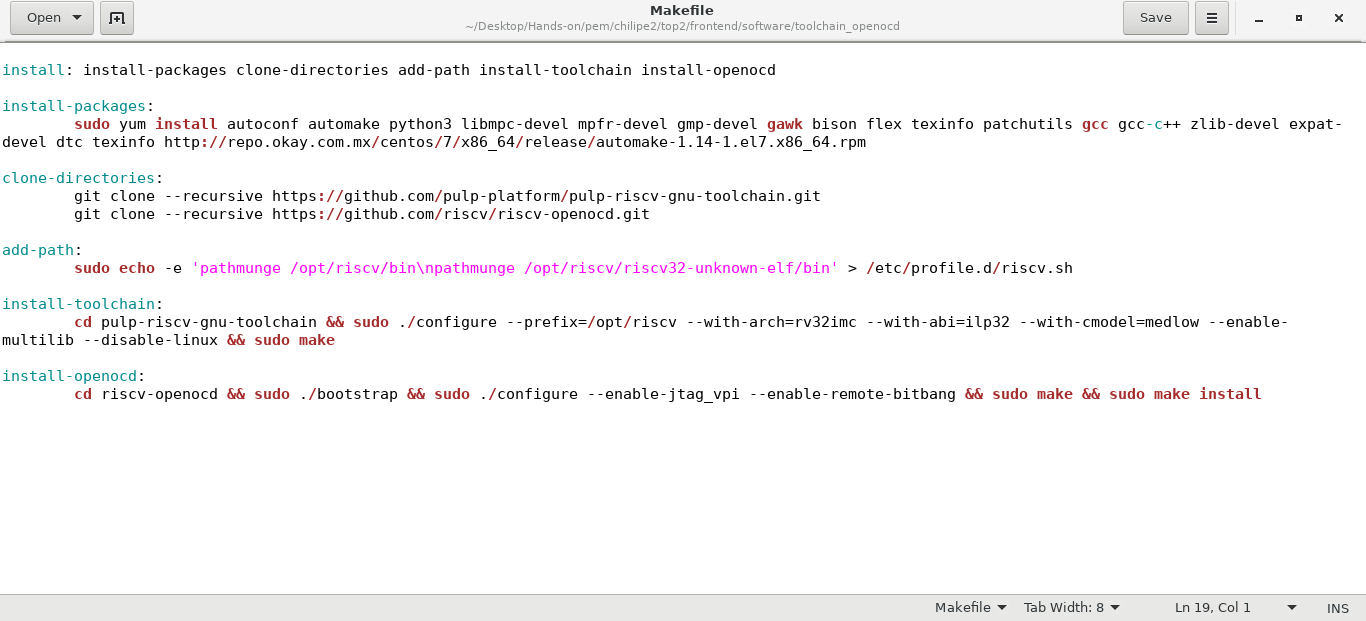
\includegraphics[width=\linewidth]{diagrams/makefile1.png}
  \caption{makefile.}
  \label{fig:top}
\end{figure}
Para rodar o makefile, recomendo não utilizar o "make install" e ir instalando linha por linha, pois pode ocorrer alguns erros; Na hora que eu rodei, deu erro na busca do repositório do openocd e do add-path, porém consegui rodar tudo no final, mesmo com esses erros.
\\	
Alguns dos comandos, podem levar até uma hora para serem executados, como é o caso dos comandos "install".


\subsection{Execução}
\par 1.Apos a instalação da toolchain, se desloque para a pasta:

\begin{itemize}
  \item cd pem/chilipe2/top2/frontend/workspace/src;
\end{itemize}

\par 2.Lá haverá um arquivo nomeado de test.c, no qual será necessário colocar o código que se deseja ser colocado no SoC.
\\
Para o propósito deste teste, um código estará contido abaixo:
\begin{lstlisting}
#define INIT_ADDR_INSTR_RAM 0x00000000
#define INIT_ADDR_DATA_RAM  0x00001000
#define INIT_ADDR_IP_RAM    0x00002000

int main()
{
	*(volatile int*) (INIT_ADDR_DATA_RAM + 0x00000000) = 0x00000030;
	*(volatile int*) (INIT_ADDR_DATA_RAM + 0x00000004) = 0x00000028;
	*(volatile int*) (INIT_ADDR_DATA_RAM + 0x00000008) = 0x00000015;
	*(volatile int*) (INIT_ADDR_DATA_RAM + 0x0000000C) = 0x00000022;
	*(volatile int*) (INIT_ADDR_DATA_RAM + 0x00000010) = 0x00000018;
	*(volatile int*) (INIT_ADDR_DATA_RAM + 0x00000014) = 0x0000004B;
	*(volatile int*) (INIT_ADDR_DATA_RAM + 0x00000018) = 0x0000004E;
	*(volatile int*) (INIT_ADDR_DATA_RAM + 0x0000001C) = 0x00000058;
	*(volatile int*) (INIT_ADDR_DATA_RAM + 0x00000020) = 0x00000004;
	*(volatile int*) (INIT_ADDR_DATA_RAM + 0x00000024) = 0x0000002B;
	*(volatile int*) (INIT_ADDR_DATA_RAM + 0x00000028) = 0x00000039;
	*(volatile int*) (INIT_ADDR_DATA_RAM + 0x0000002C) = 0x00000040;
	*(volatile int*) (INIT_ADDR_DATA_RAM + 0x00000030) = 0x00000001;
	*(volatile int*) (INIT_ADDR_DATA_RAM + 0x00000034) = 0x00000030;
	*(volatile int*) (INIT_ADDR_DATA_RAM + 0x00000038) = 0x00000038;
	*(volatile int*) (INIT_ADDR_DATA_RAM + 0x0000003C) = 0x00000002;
	*(volatile int*) (INIT_ADDR_DATA_RAM + 0x00000040) = 0x00000059;
	*(volatile int*) (INIT_ADDR_DATA_RAM + 0x00000044) = 0x0000003D;
	*(volatile int*) (INIT_ADDR_DATA_RAM + 0x00000048) = 0x00000000;
	*(volatile int*) (INIT_ADDR_DATA_RAM + 0x0000004C) = 0x00000009;
	*(volatile int*) (INIT_ADDR_DATA_RAM + 0x00000050) = 0x00000047;
	*(volatile int*) (INIT_ADDR_DATA_RAM + 0x00000054) = 0x0000002D;
	*(volatile int*) (INIT_ADDR_DATA_RAM + 0x00000058) = 0x0000005B;
	*(volatile int*) (INIT_ADDR_DATA_RAM + 0x0000005C) = 0x00000021;
	*(volatile int*) (INIT_ADDR_DATA_RAM + 0x00000060) = 0x00000005;
	*(volatile int*) (INIT_ADDR_DATA_RAM + 0x00000064) = 0x0000005E;
	*(volatile int*) (INIT_ADDR_DATA_RAM + 0x00000068) = 0x0000003E;
	*(volatile int*) (INIT_ADDR_DATA_RAM + 0x0000006C) = 0x00000047;
	*(volatile int*) (INIT_ADDR_DATA_RAM + 0x00000070) = 0x00000020;
	*(volatile int*) (INIT_ADDR_DATA_RAM + 0x00000074) = 0x00000058;
	*(volatile int*) (INIT_ADDR_DATA_RAM + 0x00000078) = 0x00000013;
	*(volatile int*) (INIT_ADDR_DATA_RAM + 0x0000007C) = 0x00000042;
	*(volatile int*) (INIT_ADDR_DATA_RAM + 0x00000080) = 0x00000023;
	*(volatile int*) (INIT_ADDR_DATA_RAM + 0x00000084) = 0x00000023;
	*(volatile int*) (INIT_ADDR_DATA_RAM + 0x00000088) = 0x0000005A;
	*(volatile int*) (INIT_ADDR_DATA_RAM + 0x0000008C) = 0x0000001C;
	*(volatile int*) (INIT_ADDR_DATA_RAM + 0x00000090) = 0x00000009;
	*(volatile int*) (INIT_ADDR_DATA_RAM + 0x00000094) = 0x00000005;
	*(volatile int*) (INIT_ADDR_DATA_RAM + 0x00000098) = 0x0000000D;
	*(volatile int*) (INIT_ADDR_DATA_RAM + 0x0000009C) = 0x0000003C;
	*(volatile int*) (INIT_ADDR_DATA_RAM + 0x000000A0) = 0x00000032;
	*(volatile int*) (INIT_ADDR_DATA_RAM + 0x000000A4) = 0x00000010;
	*(volatile int*) (INIT_ADDR_DATA_RAM + 0x000000A8) = 0x0000002D;
	*(volatile int*) (INIT_ADDR_DATA_RAM + 0x000000AC) = 0x00000020;
	*(volatile int*) (INIT_ADDR_DATA_RAM + 0x000000B0) = 0x0000002D;
	*(volatile int*) (INIT_ADDR_DATA_RAM + 0x000000B4) = 0x00000055;
	*(volatile int*) (INIT_ADDR_DATA_RAM + 0x000000B8) = 0x00000049;
	*(volatile int*) (INIT_ADDR_DATA_RAM + 0x000000BC) = 0x00000048;
	*(volatile int*) (INIT_ADDR_DATA_RAM + 0x000000C0) = 0x0000005C;
	*(volatile int*) (INIT_ADDR_DATA_RAM + 0x000000C4) = 0x0000001A;
	*(volatile int*) (INIT_ADDR_DATA_RAM + 0x000000CC) = 0x00000032; 

	int l = 1;
	while(l)
	{
		int k, j, aux;

		for (k = *(volatile int*) (INIT_ADDR_DATA_RAM + 0x000000CC) - 1; k > 0; k--)
		{
			for (j = 0; j < k; j++)
			{
				if (*(volatile int*) (INIT_ADDR_DATA_RAM + (j * 4)) > *(volatile int*) (INIT_ADDR_DATA_RAM + ((j + 1) * 4)))
				{
					*(volatile int*) (INIT_ADDR_INSTR_RAM + 0x00000FA0)   = *(volatile int*) (INIT_ADDR_DATA_RAM + (j * 4));
					*(volatile int*) (INIT_ADDR_DATA_RAM + (j * 4))       = *(volatile int*) (INIT_ADDR_DATA_RAM + ((j + 1) * 4));
					*(volatile int*) (INIT_ADDR_DATA_RAM + ((j + 1) * 4)) = *(volatile int*) (INIT_ADDR_INSTR_RAM + 0x00000FA0);
				}
			}
		}
	}
}
\end{lstlisting}

Explicando brevemente:
\\
A primeira sessão onde tem "init addr" é responsável por gerar os valores iniciais da memória de dados, os quais vão ser organizados.
\\
A segunda sessão, a partir do "while", representa um bubble sort, um algoritmo de organização,o qual será carregado na memória de instruções. Onde vai ser lido pelo core e executar a organização da memória de dados. 
\\

\par 3.Após o código ser colocado, utilize o seguinte comando para voltar uma pasta:

\begin{itemize}
  \item cd ..
\end{itemize}
\par 4.Aqui temos um Makefile, abra o terminal e digite:

\begin{itemize}
  \item make all
\end{itemize}

\par 5.Após executar do comando, 3 arquivos aparecerão na pasta:

\begin{itemize}
  \item cd pem/chilipe2/top2/frontend/rtl/tb
\end{itemize}

\begin{figure}[H]
  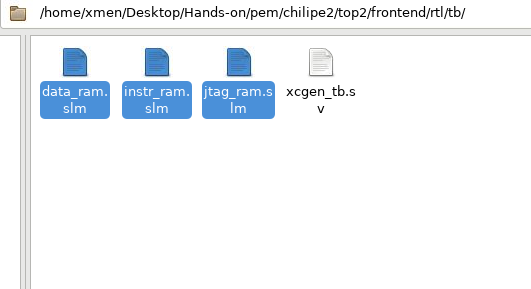
\includegraphics[width=\linewidth]{diagrams/pastatb.png}
  \caption{Arquivos na pasta tb.}
  \label{fig:top}
\end{figure}

\par 6.O arquivo é chamado jtag\_ ram\_slm , o qual vai ser lido pelo testbench, e o colocará na entrada do jtag, simulando uma interface externa e através disso, escrever nas memórias de instruções e de dados, as informações em hexadecimal, do que foi feito em C.
\\
\par 7.Agora, para a compilação do código, se dirija para :

\begin{itemize}
  \item cd ..
  \item cd ..
  \item cd scripts/rlsim
\end{itemize}

\par 8;Onde será executado os seguintes comandos:

\begin{itemize}
  \item cds
  \item make
  \item make waves
\end{itemize}

\par 9.Isto abrirá uma janela no programa "simvision" na qual será possível observer o que ocorre durante todo processo, desde a escrita nas memórias de dados e instruções através do JTAG, até a execução do código(bubble sort) pelo processador, e a organização da memória de dados através deste processo.
\\
\subsection{Faça seu teste}
Caso se deseja realizar outro teste, com diferentes endereços de memórias, é necessário alterar as informações no linker, que pode ser encontrado em:

\begin{itemize}
  \item cd pem/chilipe2/top2/frontend/workspace/tools/xcgen/ld;
\end{itemize}

Caso se deseja apenas alterar o código em C, basta alterar o código do arquivo test.c e realizar o mesmos passos (apartir do 3.)citados na sessão anterior.
\\
% subsection Hands-On (end)
